\documentclass[tikz,border=4pt]{standalone}
% Estilo común de los diagramas de bloques (se usa con \input en cada standalone)
\usepackage[defaultsans,scale=0.92]{lato}
\usepackage{libertinust1math}
\usepackage{xcolor,amsmath}
\usepackage{tikz}
\usetikzlibrary{positioning,arrows.meta,calc,shapes.geometric}
\usepackage{../../notacion}
\definecolor{ctrlazul}{HTML}{1E5AA8}\definecolor{ctrlnoche}{HTML}{14213D}
\definecolor{ctrlcoral}{HTML}{D1495B}\definecolor{ctrlverde}{HTML}{2A9D8F}
\definecolor{ctrlambar}{HTML}{E09F3E}\definecolor{ctrlgris}{HTML}{5C677D}
\definecolor{ctrlvioleta}{HTML}{6C4AB6}\definecolor{ctrlteal}{HTML}{0F7173}
\tikzset{
  >={Stealth[length=2.4mm]}, every node/.style={font=\small},
  bloque/.style={draw=ctrlnoche,fill=ctrlazul!7,thick,rounded corners=1.5pt,minimum height=9mm,minimum width=13mm,inner sep=4pt},
  suma/.style={draw=ctrlnoche,thick,circle,inner sep=0pt,minimum size=6mm},
  senal/.style={->,thick,draw=ctrlnoche},
  rot/.style={font=\footnotesize,text=ctrlgris},
}

\begin{document}
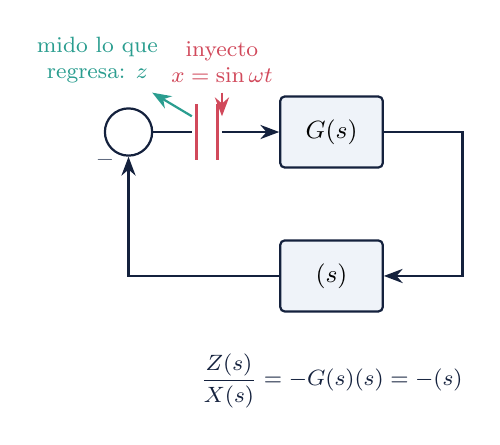
\begin{tikzpicture}[node distance=12mm]
  \node[suma] (S) {};
  \node[bloque,right=16mm of S] (G) {$G(s)$};
  \coordinate[right=10mm of G] (y0);
  \node[bloque,below=9mm of G] (H) {$\Hs(s)$};
  % corte
  \coordinate (c1) at ($(S)!0.42!(G.west)$);
  \coordinate (c2) at ($(S)!0.62!(G.west)$);
  \draw[thick,ctrlnoche] (S) -- (c1);
  \draw[senal] (c2) -- (G);
  \draw[senal] (G) -- (y0) |- (H);
  \draw[senal] (H) -| (S);
  \node[rot] at ($(S)+(-3mm,-3.5mm)$) {$-$};
  \draw[ctrlcoral,very thick] ($(c1)+(0.6mm,3.5mm)$) -- ($(c1)+(0.6mm,-3.5mm)$);
  \draw[ctrlcoral,very thick] ($(c2)+(-0.6mm,3.5mm)$) -- ($(c2)+(-0.6mm,-3.5mm)$);
  \node[ctrlcoral,above=5mm of c2,align=center,font=\footnotesize] (x) {inyecto\\ $x=\sin\omega t$};
  \draw[->,ctrlcoral,thick] (x) -- ($(c2)+(0,2mm)$);
  \node[ctrlverde,above=5mm of c1,xshift=-12mm,align=center,font=\footnotesize] (z) {mido lo que\\ regresa: $z$};
  \draw[->,ctrlverde,thick] ($(c1)+(0,2mm)$) -- (z);
  \node[below=4mm of H,font=\footnotesize,text=ctrlnoche] {$\dfrac{Z(s)}{X(s)}=-G(s)\Hs(s)=-\Gma(s)$};
\end{tikzpicture}
\end{document}
